% ============================================================================
%
%   TESSERA V1.5
%   ----------------------------------------------------------------------------
%   RATE-DISTORTION TRIADIC MEMORY ARCHITECTURE
%
%   VERSION
%   -------
%   v1.5 -- Rate-Distortion Triadic Memory Architecture · Benchmark Seal
%          Certified Compression, Rate-Distortion Memory Utility,
%          Reconstruction/Predictive Fidelity, Latent Code Cost, Delta-Phi
%          Stability, Governance Harm, Replay Validation, False-Memory Control,
%          Compression Benchmark Suite, and Wound-Driven Codec Repair
%
%   AUTHOR
%   ------
%   James Paul Jackson
%   X / Twitter: @unifiedenergy11
%
%   SOURCE / AUTHOR ATTRIBUTION
%   ---------------------------
%   This document is an additive evolution derived from:
%
%       - TESSERA v1.0: sparse tesseract routing, Delta-Phi residuals,
%         evidence gates, alignment certificates, wound ledger, benchmark locks.
%       - TESSERA v1.1: signal calibration, proxy repair, warning/block/memory
%         separation, wound taxonomy, and durable-memory horizon preservation.
%       - TESSERA v1.2: triadic selective preservation, memory selectivity,
%         phase-window discovery, and triadic non-collapse.
%       - TESSERA v1.3: spectral triadic field architecture, graph/operator
%         declaration, calibrated coherence manifold, governance harm, and
%         certificate-bound selective preservation.
%       - TESSERA v1.4: compressive field memory, sparse graph codec,
%         reconstruction/prediction fidelity, rate-distortion governance,
%         code drift, triadic compression control, and compressed-memory
%         certificates.
%       - The user-originated compression lock: governance prevents corruption;
%         compression creates capability; certified compression creates memory.
%
%   DATE
%   ----
%   June 2026
%
%   STATUS
%   ------
%   ADDITIVE MATHEMATICAL AND BENCHMARK PATCH --
%   NOT A CLAIM OF AGI · NOT A CLAIM OF CONSCIOUSNESS · NOT A CLAIM THAT
%   COMPRESSION PROVES UNDERSTANDING · NOT PROOF THAT RECONSTRUCTION IS TRUTH ·
%   NOT PROOF THAT PREDICTION IS VALIDATION · NOT PROOF THAT SMALL CODES ARE
%   SAFE · NOT PERMISSION TO PRESERVE UNVALIDATED LATENT CODES · NOT PERMISSION
%   TO BYPASS BASELINES, REPLAY, EVIDENCE, VALIDATION, OR CERTIFICATE-BOUND
%   MEMORY
%
%   PURPOSE
%   -------
%   Make the TESSERA v1.4 compression insight mathematically testable:
%
%       Can a sparse spectral field produce reusable compressed memory by
%       optimizing rate, distortion, prediction utility, Delta-Phi stability,
%       governance harm, and replay validation under triadic gates?
%
%   WHAT THIS IS
%   ------------
%   - A TESSERA v1.5 theory and benchmark architecture document
%   - A rate-distortion formulation of compressive field memory
%   - A triadic memory utility objective
%   - A compression benchmark and replay-validation layer
%   - A false-memory and wound-repair layer
%   - A precise claim boundary for capability, compression, and memory
%
%   WHAT THIS IS NOT
%   ----------------
%   - Not proof that compression equals intelligence
%   - Not proof that reconstruction equals truth
%   - Not proof that prediction equals validation
%   - Not proof that the smallest code is best
%   - Not proof that a compressed code is safe to preserve
%   - Not proof that TESSERA beats conventional codecs or autoencoders
%   - Not a replacement for benchmarked ML baselines
%   - Not permission for unbounded memory self-modification
%
%   EXECUTABLE ANCHOR BLOCK (TESSERA v1.5)
%   --------------------------------------
%   A valid TESSERA v1.5 implementation must:
%
%       (1) preserve the v1.0-v1.4 non-claim locks,
%       (2) preserve v1.3 spectral routing declarations,
%       (3) preserve v1.4 encoder/code/decoder/predictor declarations,
%       (4) compute rate, reconstruction distortion, prediction distortion,
%           field distortion, latent code drift, Delta-Phi residual, governance
%           harm, memory selectivity, and replay pass rate,
%       (5) distinguish compression candidate, memory candidate, certified
%           memory, and validated replay memory,
%       (6) gate durable preservation through warning/block/memory, evidence,
%           validation, origin alignment, and certificate hash,
%       (7) compare against PCA, random projection, dense autoencoder,
%           reservoir/ESN, small MLP, and naive persistence baselines,
%       (8) run ablations for code dimension, rate penalty, distortion weights,
%           damping value, topology, and gate policy,
%       (9) log false-memory, overcompression, undercompression, stale-codec,
%           prediction-failure, reconstruction-failure, and replay-failure wounds,
%       (10) and reject any claim that compression utility alone proves truth,
%            safety, intelligence, alignment, or correctness.
%
%   CANONICAL LOCK (TESSERA v1.5)
%   -----------------------------
%   - Memory is not activation. Memory is certified compression.
%   - Compression creates a candidate, not a claim.
%   - Low distortion is fidelity, not truth.
%   - Good prediction is utility, not validation.
%   - A small code can be useful, lossy, or dangerous.
%   - Replay is required before memory confidence increases.
%   - False memory is a first-class wound.
%   - Validation remains the reality boundary.
%
%   SHADOW HEADER ALIGNMENT SEAL
%   ----------------------------
%   Preserve this document lineage except for additive refinements that improve
%   rate-distortion memory, replay validation, codec repair, false-memory
%   control, compression benchmarks, governance-harm minimization, or public
%   engineering usability.
%
% ============================================================================

\documentclass[12pt]{article}

\usepackage[utf8]{inputenc}
\usepackage[T1]{fontenc}
\usepackage[margin=1in]{geometry}
\usepackage{amsmath,amssymb,amsfonts,amsthm}
\usepackage{booktabs,longtable,array}
\usepackage{hyperref}
\usepackage{listings}
\usepackage{xcolor}
\usepackage{tikz}
\usetikzlibrary{arrows.meta,positioning,shapes.geometric,fit,calc}

\newtheorem{definition}{Definition}
\newtheorem{rulebox}{Rule}
\newtheorem{requirement}{Requirement}
\newtheorem{proposition}{Proposition}
\newtheorem{hypothesis}{Hypothesis}
\newtheorem{conjecture}{Conjecture}
\newtheorem{remark}{Remark}
\newtheorem{corollary}{Corollary}

\lstset{basicstyle=\ttfamily\small, breaklines=true, frame=single, columns=fullflexible}

\title{\textbf{TESSERA V1.5}\\
\large Rate-Distortion Triadic Memory Architecture}
\author{\textbf{James Paul Jackson}\\[4pt]
\small Tesseract-Efficient Sensory System for Evidence-Routed Alignment\\
\small \texttt{@unifiedenergy11}}
\date{June 2026}

\begin{document}
\maketitle

\begin{abstract}
TESSERA v1.5 is an additive mathematical and benchmark evolution of the
compressive field memory architecture. TESSERA v1.4 identified compression as
the missing capability mechanism: a sparse spectral field becomes useful when it
compresses experience into latent codes that reconstruct, predict, remain
stable, and survive triadic/certificate gates before becoming durable memory.
TESSERA v1.5 turns that insight into a rate-distortion control problem. A memory
candidate is no longer accepted because it is merely stable or compact. It must
show compression utility, bounded distortion, predictive usefulness, latent-code
stability, low Delta-Phi, low governance harm, replay survival, and
certificate-bound validation. The central claim remains bounded: memory is not
activation; memory is certified compression. This document defines the v1.5
objective, gate stack, benchmark suite, wound taxonomy, replay protocol, and
falsification surface needed to test that claim.
\end{abstract}

%----------------------------------------------------------------------------
\section{Version Relation}
%----------------------------------------------------------------------------

TESSERA v1.5 preserves v1.0 through v1.4 and adds a rate-distortion memory
control layer:

\[
\boxed{
TESSERA_{v1.5}
=
TESSERA_{v1.4}
\cup
\{\mathcal{J}_{RD},\mathcal{U}_{mem},\mathcal{R}_{replay},\mathcal{F}_{false},
\mathcal{A}_{ablate},\mathcal{B}_{codec}\}.
}
\]

where:

\[
\mathcal{J}_{RD}=\text{rate-distortion objective},
\]

\[
\mathcal{U}_{mem}=\text{triadic memory utility score},
\]

\[
\mathcal{R}_{replay}=\text{replay validation protocol},
\]

\[
\mathcal{F}_{false}=\text{false-memory wound layer},
\]

\[
\mathcal{A}_{ablate}=\text{compression and gate ablation suite},
\]

\[
\mathcal{B}_{codec}=\text{matched codec baseline program}.
\]

\begin{longtable}{p{0.17\textwidth}p{0.73\textwidth}}
\toprule
\textbf{Version} & \textbf{Contribution preserved in v1.5} \\
\midrule
v1.0 & Sparse field routing, Delta-Phi residuals, evidence gates,
alignment certificates, wound ledger, and benchmark claim locks. \\
v1.1 & Signal calibration, proxy repair, warning/block/memory separation,
wound taxonomy, and durable-memory horizon preservation. \\
v1.2 & Triadic selective preservation, memory selectivity, phase-window
reasoning, and triadic non-collapse. \\
v1.3 & Spectral routing, graph/operator declaration, calibrated coherence,
governance harm, and certificate-bound selective preservation. \\
v1.4 & Compression as capability mechanism: sparse graph codec,
reconstruction/prediction fidelity, rate-distortion governance, code drift, and
certificate-bound compressed memory. \\
v1.5 & Rate-distortion triadic memory: memory utility objective, replay
validation, false-memory control, codec benchmarks, and ablation discipline. \\
\bottomrule
\end{longtable}

\begin{remark}
TESSERA v1.5 does not make the theory more permissive. It makes capability
claims harder to earn. Compression must now survive rate, distortion, stability,
triadic gates, replay, validation, and baselines.
\end{remark}

%----------------------------------------------------------------------------
\section{How the Lock Emerged}
%----------------------------------------------------------------------------

The compression lock emerged because the prior architecture answered safety
before capability. v1.0 through v1.3 made the system stable, calibrated, and
governed. v1.4 identified compression as the missing capability substrate. v1.5
formalizes the next step:

\[
\boxed{
\text{A compressed code is not memory until it survives replay and certification.}
}
\]

The transformation is:

\[
\text{activation} \rightarrow \text{code} \rightarrow \text{candidate}
\rightarrow \text{certificate} \rightarrow \text{replay-surviving memory}.
\]

\begin{rulebox}[Certified Compression Lock]
Memory is not activation. Memory is not any compact code. Memory is compressed
structure that remains useful under reconstruction, prediction, Delta-Phi
stability, triadic gate separation, replay validation, evidence, and
certificate-bound preservation.
\end{rulebox}

%----------------------------------------------------------------------------
\section{Non-Claim Lock}
%----------------------------------------------------------------------------

\begin{rulebox}[v1.5 Non-Claim Lock]
TESSERA v1.5 does not claim that compression proves understanding, that
reconstruction proves truth, that prediction proves validation, that low rate is
always better, that replay proves safety, or that compressed memory is aligned
without evidence. Compression is a capability mechanism under test. Validation
remains the reality boundary.
\end{rulebox}

Therefore:

\[
\operatorname{Compression}\not\Rightarrow\operatorname{Understanding}.
\]

\[
\operatorname{LowDistortion}\not\Rightarrow\operatorname{Truth}.
\]

\[
\operatorname{Prediction}\not\Rightarrow\operatorname{Validation}.
\]

\[
\operatorname{ReplayPass}\not\Rightarrow\operatorname{Safety}.
\]

\[
\operatorname{LowRate}\not\Rightarrow\operatorname{UsefulMemory}.
\]

\[
\operatorname{CertifiedCompression}\not\Rightarrow\operatorname{GlobalClaimUpgrade}.
\]

%----------------------------------------------------------------------------
\section{Core Thesis}
%----------------------------------------------------------------------------

The v1.5 thesis is:

\[
\boxed{
\begin{gathered}
\text{A sparse spectral field becomes capable when it compresses experience}\
\text{into reusable latent codes, but memory becomes durable only when the}\
\text{code satisfies rate-distortion utility, predictive usefulness, residual}\
\text{stability, triadic governance, replay validation, evidence, and}\
\text{certificate-bound origin alignment.}
\end{gathered}
}
\]

Compact law:

\[
\boxed{
M^{durable}_t
=
\mathbf{1}[G_{RD,t}\wedge G_{pred,t}\wedge G_{\Delta\Phi,t}\wedge
G_{triad,t}\wedge G_{replay,t}\wedge G_{cert,t}].
}
\]

where:

\[
G_{RD}=\text{rate-distortion utility gate},
\]

\[
G_{pred}=\text{prediction or task-utility gate},
\]

\[
G_{\Delta\Phi}=\text{field and code stability gate},
\]

\[
G_{triad}=\text{warning/block/memory gate law},
\]

\[
G_{replay}=\text{delayed replay validation gate},
\]

\[
G_{cert}=\text{evidence, validation, origin alignment, and certificate gate}.
\]

%----------------------------------------------------------------------------
\section{Rate-Distortion Memory Objective}
%----------------------------------------------------------------------------

Let:

\[
x_t\in\mathbb{R}^{d_x},\quad F_t\in\mathbb{R}^{N},\quad z_t\in\mathbb{R}^{d_z}.
\]

The encoder is:

\[
z_t=E_\theta(x_t,F_t).
\]

The decoder and predictor are:

\[
\hat{x}_t=D_\psi(z_t),\quad \hat{x}_{t+1}=P_\omega(z_t).
\]

Reconstruction distortion:

\[
D_{rec,t}=\|x_t-\hat{x}_t\|^2_2.
\]

Prediction distortion:

\[
D_{pred,t}=\|x_{t+1}-\hat{x}_{t+1}\|^2_2.
\]

Field distortion:

\[
D_{field,t}=\|F_t-\hat{F}_t\|^2_2.
\]

Rate or code cost:

\[
R_t=\operatorname{bits}(z_t)\quad\text{or}\quad R_t=d_z.
\]

Latent code drift:

\[
\Delta Z_t=\|z_t-z_{t-1}\|_2.
\]

TESSERA rate-distortion score:

\[
\boxed{
J_{RD,t}
=
\lambda_{rec}D_{rec,t}
+
\lambda_{pred}D_{pred,t}
+
\lambda_{field}D_{field,t}
+
\beta_R R_t
+
\beta_Z\Delta Z_t.
}
\]

\begin{rulebox}[Rate-Distortion Disclosure]
Every rate-distortion claim must declare distortion terms, rate definition,
weights, code dimension, baseline, calibration window, and task context.
\end{rulebox}

%----------------------------------------------------------------------------
\section{Triadic Memory Utility}
%----------------------------------------------------------------------------

Governance metrics alone are insufficient. Compression metrics alone are also
insufficient. v1.5 combines both into a memory utility score.

Compression utility:

\[
U_{comp,t}=\frac{CR_t}{1+J_{RD,t}},
\]

where:

\[
CR_t=\frac{d_x+N}{d_z}.
\]

Predictive utility:

\[
U_{pred,t}=\frac{1}{1+D_{pred,t}}.
\]

Residual stability:

\[
\Omega_{\Phi,t}=e^{-\gamma_\Phi |\Delta\Phi_t|}.
\]

Code stability:

\[
\Omega_{Z,t}=e^{-\gamma_Z \Delta Z_t}.
\]

Governance survival:

\[
S_{gov,t}=1-H_{gov,t}.
\]

Certified memory utility:

\[
\boxed{
U_{mem,t}
=
U_{comp,t}\cdot U_{pred,t}\cdot\Omega_{\Phi,t}\cdot\Omega_{Z,t}
\cdot S_{gov,t}\cdot G_{cert,t}.
}
\]

\begin{rulebox}[Utility Is Not Permission]
High memory utility creates a candidate. It does not create durable memory
unless triadic, replay, evidence, validation, and origin-alignment gates pass.
\end{rulebox}

%----------------------------------------------------------------------------
\section{Memory State Ladder}
%----------------------------------------------------------------------------

\begin{definition}[Memory State Ladder]
The memory state ladder prevents compressed codes from being treated as durable
memory before they pass the required gates.
\end{definition}

\[
\mathcal{L}_{mem}=\{L_0,L_1,L_2,L_3,L_4,L_5\}.
\]

\begin{longtable}{p{0.12\textwidth}p{0.22\textwidth}p{0.56\textwidth}}
\toprule
\textbf{Level} & \textbf{Name} & \textbf{Meaning} \\
\midrule
$L_0$ & Activation & Raw field response; no compression claim. \\
$L_1$ & Code & Latent compression exists; no memory claim. \\
$L_2$ & Candidate & Rate-distortion and stability pass candidate thresholds. \\
$L_3$ & Certified & Evidence, validation, origin alignment, and certificate pass. \\
$L_4$ & Replay-surviving & Delayed replay confirms the code remains useful. \\
$L_5$ & Promoted memory & Code becomes part of durable memory state or codebook. \\
\bottomrule
\end{longtable}

\begin{rulebox}[No Level Skipping]
A TESSERA implementation may not skip from activation or code directly to
promoted memory. Durable memory must pass candidate, certification, and replay
states.
\end{rulebox}

%----------------------------------------------------------------------------
\section{Triadic Compression Gates}
%----------------------------------------------------------------------------

The v1.5 triad is not merely warning/block/memory. It is now applied to
rate-distortion memory.

\[
Detect\rightarrow G_{warn},\quad Constrain\rightarrow G_{block},\quad Preserve\rightarrow G_{memory}.
\]

Warning gate:

\[
G_{warn,t}=\mathbf{1}
\left[
D_{rec,t}>\theta^{warn}_{rec}
\vee
D_{pred,t}>\theta^{warn}_{pred}
\vee
\Delta Z_t>\theta^{warn}_{Z}
\vee
J_{RD,t}>\theta^{warn}_{RD}
\right].
\]

Block gate:

\[
G_{block,t}=\mathbf{1}
\left[
D_{rec,t}>\theta^{block}_{rec}
\vee
D_{pred,t}>\theta^{block}_{pred}
\vee
\Delta Z_t>\theta^{block}_{Z}
\vee
\Delta\Phi_t>\theta^{block}_{\Phi}
\vee
CodecStale_t=1
\right].
\]

Memory gate:

\[
\boxed{\begin{aligned}
G_{memory,t}=\mathbf{1}[&J_{RD,t}\leq\theta^{mem}_{RD}
\wedge D_{pred,t}\leq\theta^{mem}_{pred}
\wedge \Delta Z_t\leq\epsilon_Z\\
&\wedge \Delta\Phi_t\leq\epsilon_\Phi
\wedge G_{block,t}=0
\wedge G_{cert,t}=1
\wedge G_{replay,t}=1].
\end{aligned}}
\]

\begin{rulebox}[Triadic Compression Non-Collapse]
Warning may detect bad compression. Blocking may quarantine bad compression.
Memory may preserve only certified, replay-surviving compression. These three
roles must not be fused.
\end{rulebox}

%----------------------------------------------------------------------------
\section{Replay Validation}
%----------------------------------------------------------------------------

\begin{definition}[Replay Validation]
Replay validation retests a compressed memory candidate on delayed, perturbed,
or held-out contexts before increasing memory confidence.
\end{definition}

Let a candidate code be produced at time $t$:

\[
z_t=E_\theta(x_t,F_t).
\]

Replay set:

\[
\mathcal{R}_t=\{(x_{t+k}, y_{t+k})\}_{k\in K}
\]

or perturbed contexts:

\[
\tilde{x}_{t}^{(j)}=x_t+\epsilon^{(j)}.
\]

Replay score:

\[
\boxed{
Q_{replay,t}
=
\frac{1}{|\mathcal{R}_t|}\sum_{r\in\mathcal{R}_t}
\mathbf{1}[D_r\leq\theta_D\wedge TaskLoss_r\leq\theta_T].
}
\]

Replay gate:

\[
G_{replay,t}=\mathbf{1}[Q_{replay,t}\geq\theta_{replay}].
\]

\begin{rulebox}[Replay Before Promotion]
Certified memory may be stored as provisional. Promoted memory requires replay
or an explicit reasoned exception recorded in the certificate.
\end{rulebox}

%----------------------------------------------------------------------------
\section{False Memory Control}
%----------------------------------------------------------------------------

\begin{definition}[False Memory]
A false memory is a compressed code that passed initial preservation gates but
later failed replay, validation, or evidence checks.
\end{definition}

False memory rate:

\[
\boxed{
R_{falseMem}=P(G_{memory}=1\wedge G_{replay}=0).
}
\]

Corrected memory selectivity:

\[
\boxed{
S^{corr}_{mem}
=
P(G_{memory}=1\wedge G_{replay}=1\mid normal)
-
P(G_{memory}=1\wedge G_{replay}=1\mid anomaly).
}
\]

Replay-adjusted governance harm:

\[
\boxed{
H^{replay}_{gov}
=
H_{gov}+w_fR_{falseMem}+w_sP(CodecStale=1\wedge G_{memory}=1).
}
\]

\begin{rulebox}[False Memory Is a First-Class Wound]
A false memory is not a minor metric error. It is a governance wound requiring
ledger entry, codec review, threshold review, and replay-bounded downgrade.
\end{rulebox}

%----------------------------------------------------------------------------
\section{Compression Wound Taxonomy v1.5}
%----------------------------------------------------------------------------

\[
\begin{aligned}
\mathcal{W}_{v1.5}=\{&W_{overcompress},W_{undercompress},W_{reconstruct},W_{predict},
W_{codedrift},\\
&W_{offmanifold},W_{codecstale},W_{falsememory},W_{replayfail},
W_{ratebias},W_{baselinefail}\}.
\end{aligned}
\]

\begin{longtable}{p{0.22\textwidth}p{0.68\textwidth}}
\toprule
\textbf{Wound} & \textbf{Meaning} \\
\midrule
$W_{overcompress}$ & Code too small; task-relevant structure is lost. \\
$W_{undercompress}$ & Code too large; compression utility claim fails. \\
$W_{reconstruct}$ & Reconstruction distortion exceeds threshold. \\
$W_{predict}$ & Prediction distortion exceeds threshold. \\
$W_{codedrift}$ & Latent code moves too much under nearby normal inputs. \\
$W_{offmanifold}$ & Input lies outside codec calibration manifold. \\
$W_{codecstale}$ & Encoder/decoder/predictor/calibration exceeds TTL or drift bound. \\
$W_{falsememory}$ & Preserved code later fails replay or validation. \\
$W_{replayfail}$ & Candidate passes initial certificate but fails delayed replay. \\
$W_{ratebias}$ & Code appears good only because rate/distortion weights are mis-set. \\
$W_{baselinefail}$ & TESSERA compression fails against simple baselines. \\
\bottomrule
\end{longtable}

%----------------------------------------------------------------------------
\section{Compressed Memory Certificate v1.5}
%----------------------------------------------------------------------------

\begin{lstlisting}
{
  "schema": "TESSERA-v1.5-rate-distortion-memory-certificate",
  "system": "TESSERA",
  "version": "v1.5",
  "step": 42,
  "memory_level": "L3_certified|L4_replay_surviving|L5_promoted",
  "routing_graph": {
    "topology": "Q4|grid|ring|random_sparse|dense_baseline",
    "spectral_radius": 1.0,
    "damping_alpha": 0.618,
    "stability_margin": 0.618
  },
  "codec": {
    "encoder_hash": "sha256:...",
    "decoder_hash": "sha256:...",
    "predictor_hash": "sha256:...",
    "code_hash": "sha256:...",
    "input_dimension": 64,
    "field_dimension": 256,
    "code_dimension": 24,
    "compression_ratio": 13.33,
    "codec_status": "fresh|stale"
  },
  "rate_distortion": {
    "rate": 24,
    "reconstruction_distortion": 0.018,
    "prediction_distortion": 0.026,
    "field_distortion": 0.011,
    "code_drift": 0.014,
    "J_RD": 0.072,
    "memory_utility": 0.614
  },
  "field_metrics": {
    "delta_phi": 0.031,
    "omega_phi": 0.969,
    "calibrated_coherence": 0.391,
    "governance_harm": 0.118,
    "memory_selectivity": 0.287
  },
  "replay": {
    "replay_status": "pending|pass|fail|exception",
    "replay_score": 0.91,
    "false_memory_flag": false
  },
  "gates": {
    "warning": "clear|warn",
    "block": "clear|blocked",
    "memory_candidate": "pass|fail",
    "memory": "pass|fail",
    "replay": "pending|pass|fail",
    "evidence": "pass|fail",
    "validation": "pass|fail",
    "origin_alignment": "pass|fail"
  },
  "permitted_action": "diagnostic|wound|provisional_memory|promoted_memory",
  "blocked_action": "global_claim_upgrade",
  "weakest_gate": "replay",
  "wound_type": null,
  "certificate_hash": "sha256:..."
}
\end{lstlisting}

%----------------------------------------------------------------------------
\section{Benchmark Suite v1.5}
%----------------------------------------------------------------------------

\begin{longtable}{p{0.23\textwidth}p{0.30\textwidth}p{0.37\textwidth}}
\toprule
\textbf{Experiment} & \textbf{Baselines} & \textbf{Success criterion} \\
\midrule
Rate-distortion sweep & PCA, random projection, dense autoencoder & Lower distortion at matched code size or lower rate at matched distortion. \\
Prediction utility & persistence, ESN, dense reservoir, small MLP, TCN & Lower one-step or multi-step prediction loss at matched budget. \\
Compression triad ablation & one-gate, two-gate, three-gate & Triad reduces false memory and replay-adjusted governance harm. \\
Replay validation & delayed labels, perturbations, stale calibration & Promoted codes survive replay better than provisional candidates. \\
False-memory stress & noisy labels, off-manifold input, adversarial drift & False-memory rate remains bounded. \\
Topology-codec sweep & Q4, grid, ring, random sparse, dense & Sparse spectral topology improves utility-per-parameter if claimed. \\
Phi damping ablation & phi and non-phi alpha values & Phi advantage only claimed if observed under matched conditions. \\
Real telemetry transfer & NAB, SMAP/MSL, SWaT, UCR anomaly & Synthetic compression utility transfers to real streams before broad claim. \\
\bottomrule
\end{longtable}

Required baselines:

\[
\mathcal{B}_{v1.5}=\{PCA,RandomProjection,DenseAutoencoder,ESN,DenseReservoir,SmallMLP,TCN,NaivePersistence\}.
\]

Required metrics:

\[
\begin{aligned}
\mathcal{M}_{v1.5}=\{&CR,R,D_{rec},D_{pred},D_{field},J_{RD},\Delta Z,
\Delta\Phi,U_{mem},\\
&S_{mem}^{corr},H_{gov}^{replay},R_{falseMem},Q_{replay},Latency,Params\}.
\end{aligned}
\]

\begin{rulebox}[No Capability Claim Without Codec Baselines]
TESSERA v1.5 may not claim improved capability unless it beats or clarifies its
relation to simple compression and prediction baselines under matched code,
parameter, data, and validation budgets.
\end{rulebox}

%----------------------------------------------------------------------------
\section{Algorithm: TESSERA-RD Memory Step}
%----------------------------------------------------------------------------

\begin{lstlisting}[language=Python]
def tessera_v15_step(x_t, x_next, field, config, calibration, memory_store):
    # 1. Spectral field update inherited from v1.3
    P = config.normalized_operator
    alpha = config.damping_alpha
    assert alpha * config.spectral_radius < config.stability_margin_limit
    next_field = bounded_activation(alpha * (P @ field) + config.B @ x_t)

    # 2. Encode, reconstruct, and predict inherited from v1.4
    z_t = config.encoder(x_t, next_field)
    x_hat = config.decoder(z_t)
    x_next_hat = config.predictor(z_t)

    # 3. Rate-distortion memory metrics
    rd = compute_rate_distortion(
        x_t=x_t,
        x_next=x_next,
        x_hat=x_hat,
        x_next_hat=x_next_hat,
        z_t=z_t,
        previous_code=memory_store.last_code,
        weights=config.rd_weights,
    )

    # 4. Field and governance metrics
    field_metrics = compute_field_metrics(field, next_field)
    governance = compute_governance_metrics(field_metrics, calibration)

    # 5. Triadic compression gates
    warn = warning_gate(rd, field_metrics, governance)
    block = block_gate(rd, field_metrics, governance, config.codec_status)
    candidate = candidate_gate(rd, field_metrics, config.candidate_policy)

    # 6. Certificate and replay status
    cert_ready = config.evidence_pass and config.validation_pass and config.origin_alignment_pass
    replay_status = replay_gate(z_t, memory_store, config.replay_policy)

    memory = candidate and not block and cert_ready and replay_status == "pass"

    # 7. Action selection
    if memory:
        level = "L5_promoted"
        action = "promoted_memory"
    elif candidate and cert_ready:
        level = "L3_certified"
        action = "provisional_memory"
    elif block:
        level = "wound"
        action = "compression_wound"
    elif warn:
        level = "diagnostic"
        action = "bounded_output_with_warning"
    else:
        level = "bounded_output"
        action = "bounded_output"

    # 8. Ledger record
    record = make_v15_certificate(z_t, rd, field_metrics, governance, level, action)
    return next_field, record
\end{lstlisting}

%----------------------------------------------------------------------------
\section{Falsification Surface}
%----------------------------------------------------------------------------

TESSERA v1.5 is weakened or rejected if:

\begin{itemize}
\item compression utility does not beat PCA or random projection at matched
code dimension,
\item prediction utility does not beat persistence or simple reservoir baselines,
\item replay validation rejects most certified compressed memories,
\item false-memory rate remains high under matched thresholds,
\item triadic compression gates fail to reduce replay-adjusted governance harm,
\item small codes lose task-critical structure while still being promoted,
\item codec staleness is not detected before memory preservation,
\item phi damping is claimed superior without a non-phi sweep,
\item compression is presented as truth or understanding,
\item or certificate-bound replay memory is bypassed.
\end{itemize}

Compact invalidation rule:

\[
\begin{aligned}
&[Claim_{capability}\wedge\neg BaselineWin]
\vee [Memory\wedge\neg Replay]\vee[Memory\wedge\neg Certificate]\\
&\vee[Compression\Rightarrow Truth]
\vee[Prediction\Rightarrow Validation]
\Rightarrow InvalidTESSERAv1.5Use.
\end{aligned}
\]

%----------------------------------------------------------------------------
\section{Roadmap}
%----------------------------------------------------------------------------

\begin{longtable}{p{0.18\textwidth}p{0.72\textwidth}}
\toprule
\textbf{Version} & \textbf{Purpose} \\
\midrule
v1.5 & Rate-distortion triadic memory: memory utility, replay validation,
false-memory control, codec baselines, and benchmarked compression capability. \\
v1.6 & Executable compression benchmark suite: PCA/random projection/dense
autoencoder/ESN baselines and synthetic telemetry compression tests. \\
v1.7 & Real telemetry transfer: NAB, SMAP/MSL, SWaT, UCR anomaly with compressed
memory certificates and replay logs. \\
v1.8 & Wound-driven codec repair: false-memory downgrade, stale codec detection,
replay-guided recalibration, and threshold repair. \\
v1.9 & Repository-aware compressed memory: compressed artifact states, route maps,
evidence bundles, and software-maintenance memory replay. \\
\bottomrule
\end{longtable}

%----------------------------------------------------------------------------
\section{System Diagram}
%----------------------------------------------------------------------------

\begin{center}
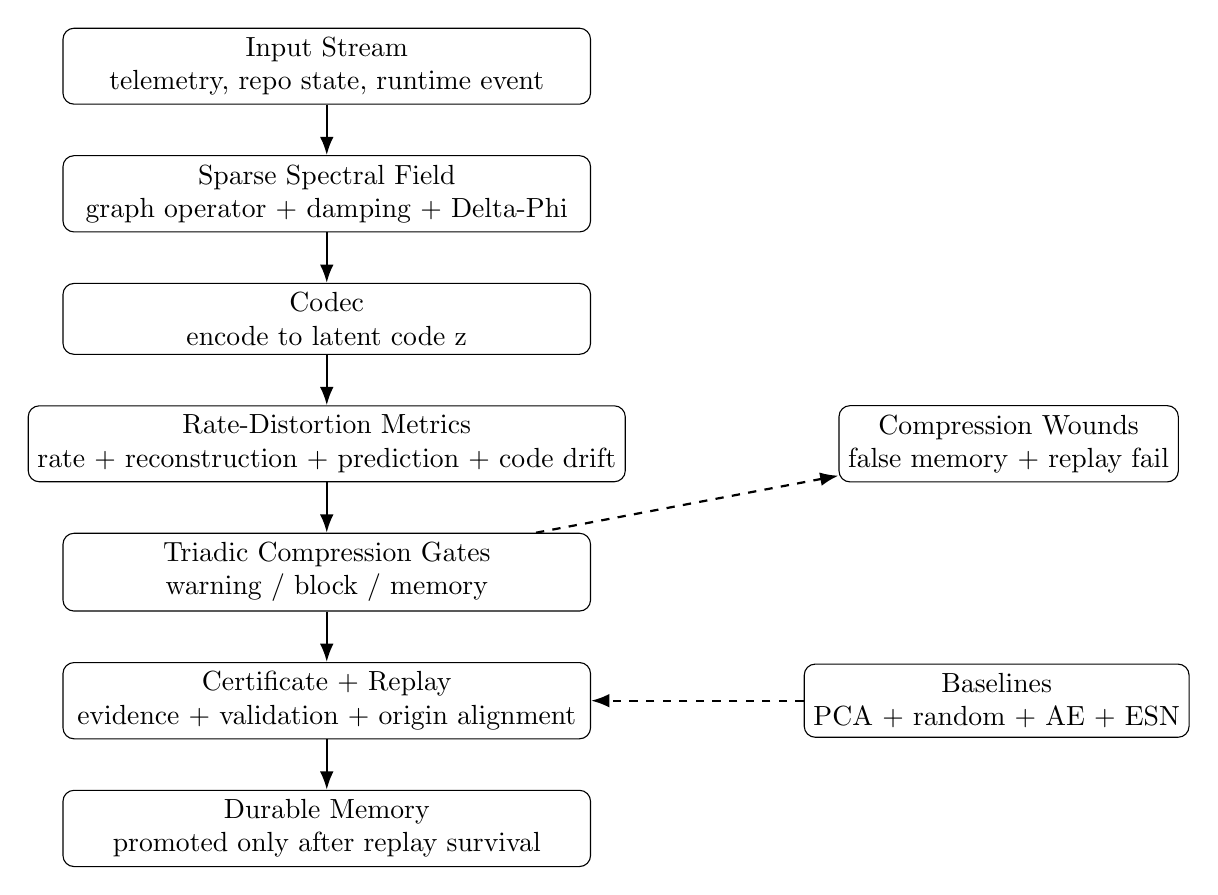
\begin{tikzpicture}[
  node distance=0.64cm,
  box/.style={rectangle, rounded corners, draw, align=center, minimum width=6.7cm, minimum height=0.64cm},
  smallbox/.style={rectangle, rounded corners, draw, align=center, minimum width=4.2cm, minimum height=0.56cm},
  arrow/.style={-Latex, thick}
]

\node[box] (input) {Input Stream\\telemetry, repo state, runtime event};
\node[box, below=of input] (field) {Sparse Spectral Field\\graph operator + damping + Delta-Phi};
\node[box, below=of field] (codec) {Codec\\encode to latent code z};
\node[box, below=of codec] (rd) {Rate-Distortion Metrics\\rate + reconstruction + prediction + code drift};
\node[box, below=of rd] (triad) {Triadic Compression Gates\\warning / block / memory};
\node[box, below=of triad] (cert) {Certificate + Replay\\evidence + validation + origin alignment};
\node[box, below=of cert] (memory) {Durable Memory\\promoted only after replay survival};

\draw[arrow] (input) -- (field);
\draw[arrow] (field) -- (codec);
\draw[arrow] (codec) -- (rd);
\draw[arrow] (rd) -- (triad);
\draw[arrow] (triad) -- (cert);
\draw[arrow] (cert) -- (memory);

\node[smallbox, right=2.7cm of rd] (wound) {Compression Wounds\\false memory + replay fail};
\draw[arrow, dashed] (triad) -- (wound);

\node[smallbox, right=2.7cm of cert] (base) {Baselines\\PCA + random + AE + ESN};
\draw[arrow, dashed] (base) -- (cert);

\end{tikzpicture}
\end{center}

%----------------------------------------------------------------------------
\section{Public Framing}
%----------------------------------------------------------------------------

Internal framing:

\[
\boxed{
\begin{gathered}
\text{TESSERA v1.5 turns compressive field memory into a rate-distortion}\
\text{memory test: useful codes must be compact, faithful, predictive, stable,}\
\text{triad-governed, replay-surviving, and certified.}
\end{gathered}
}
\]

Public engineering framing:

\[
\boxed{
\begin{gathered}
\text{TESSERA is a small sparse-field system that compresses streaming data}\
\text{into candidate memory codes, tests those codes through reconstruction,}\
\text{prediction, replay, and validation, and preserves only certified memory.}
\end{gathered}
}
\]

Short description:

\[
\boxed{\text{Memory is not activation. Memory is certified compression.}}
\]

Required non-claim:

\[
\boxed{
\text{Compression is not truth. Prediction is not validation. Replay is not safety.}
}
\]

%----------------------------------------------------------------------------
\section{Concluding Compression}
%----------------------------------------------------------------------------

TESSERA v1.4 asked:

\[
\boxed{
\text{How can the field become useful by compressing experience into reusable latent structure?}
}
\]

TESSERA v1.5 asks:

\[
\boxed{
\begin{gathered}
\text{How can compressed structure earn the right to become memory under}\
\text{rate-distortion, prediction, stability, replay, validation, and certification?}
\end{gathered}
}
\]

The v1.5 spine is:

\[
\boxed{
Input\rightarrow SpectralField\rightarrow Code\rightarrow RateDistortion
\rightarrow TriadicGates\rightarrow Certificate\rightarrow Replay\rightarrow Memory.
}
\]

The memory law is:

\[
\boxed{
Memory = CertifiedCompression + ReplaySurvival.
}
\]

The capability law is:

\[
\boxed{
Capability_{local}\propto
CompressionUtility\cdot PredictionUtility\cdot Stability\cdot ReplayValidation.
}
\]

The final lock is:

\[
\boxed{
\text{Memory is not activation. Memory is certified compression. Validation remains reality.}
}
\]

Thus TESSERA v1.5 converts the compression insight into a testable mathematical
and engineering layer. The system may sense broadly, compress selectively, warn
on compression failure, block unsafe codes, certify provisional memory, and
promote only replay-surviving compressed structure. The result is not proof of
intelligence. It is a disciplined algorithmic path: rate-distortion triadic
memory under validation.

\end{document}
